\section{Lecture 1: Ionic and Covalent Compounds}
\textbf{References chapter 5 of the textbook.}

\subsection{Types of Chemical Bonds}

There are two main types of chemical compounds: ionic compounds and molecular compounds. \\

\noindent
\note{The attractive forces that hold atoms together are called chemical bonds.}

\begin{defn}
An ionic bond is a chemical bond formed through the tranfer of electrons from one atom (or group of atoms) to another to form ions. A covalent bond is a chemical bond formed through the sharing of electron \textbf{pairs} between atoms.
\end{defn}

\begin{table}[H]
\noindent\makebox[\textwidth]{
\begin{tabular}{|l|p{0.4\textwidth}|p{0.4\textwidth}|}
\hline
\textbf{Property} & \textbf{Ionic Bond} & \textbf{Covalent Bond} \\
\hline
Chemical Formula & Formula Unit & Molecular Formula \\
\hline
Molecule Discreteness & No Discrete Molecule & Forms Discrete Molecules \\
\hline
Melting Point & High Melting Point & Lower Melting Points \\
\hline
Electrical Conductivity & Good Conductors when Molten & Cannot Conduct \\
\hline
Solubility & Soluble in Polar Solvents and Not Soluble in Non-Polar Solvents & Soluble in Non-Polar Solvents and Some Polar Solvents \\
\hline
State of Matter & N/A & Gases, Liquids, and Low-Melting Solids \\
\hline
\end{tabular}}
\end{table}

\noindent
\note{Chemical bonds can be strongly ionic or strongly covalent, but they will usually be a mix of both.} \\

\noindent
\note{Only valence electrons are able to be utilized for bonding.} \\

\subsubsection{The Octet Rule}

Electron bonds occur to further stabilize a chemical or group of chemicals by reaching a state of completely full valence electrons. Thus, Noble Gases are entirely unreactive, as they already have completely full valence electrons. Through these bonds, electrons can either \textbf{lose, gain, or share} electrons to reach a full valence state (which would be the same configuration as any one of the noble gases). This process is often referred to as \textbf{the octet rule.}

\subsubsection{Lewis Dot Symbols}

\begin{defn}
A Lewis Dot Symbol is a chemical symbol of an element surrounded by dots equal to the number of valence electrons.
\end{defn}

\noindent
\note{The choice of where the dots are placed is not important.}

\subsection{Ionic Bonds}

\begin{defn}
Ions are atoms (or groups of atoms) that are electrically charged as the result of losing or gaining valence electrons. Anions are negatively charged (usually nonmetals), and cations are positively charged (usually metals).
\end{defn}

\noindent
Whether or not an element loses or gains electrons is dependent on how many valence electrons the element has. If the number of valence electrons is closer to 0, it is more likely to lose electrons, and if the number of valence electrons is closer to 8, it is more likely to gain electrons.  \\

\noindent
This property is why metals, which are generally closer to the left of the periodic table and thus have less valence electrons, are more likely to lose electrons, and non-metals, which are further to the right and thus have more valence electrons, and more likely to gain electrons. \\

\noindent
\note{By this rule, common ionic behavior is best observed in the representative elements (but not in the transition elements, as they have a more balanced number of valence electrons). Group 1 will normally have a 1+ charge, group 2 will normally have a 2+ charge, group 13 will have a 3+ charge, group 14 will have a 4+ or 4- charge, group 15 will have a 3- charge, group 16 will have a 2- charge, and group 17 will have a 1- charge.} \\

\noindent
Ions with the same electron configuration as a noble gas are considered \textbf{Isoelectronic} with athe noble gas, and \textbf{isoelectronic species} are the set of ions (and possibly an element as well) that all have the same electron configuration.

\subsubsection{Ionic Compound Formulas}

The net charge of every compound must be equal to zero, with positive ions written first and negative ions written after. Charges on each individual ions are not reflected in the formula, and subscript numbers in the formula give the combining ratio of the ions rather than the exact count. \\

\noindent
For example, in the ion \ce{NaCl}, Na carries a +1 charge and Cl carries a -1 charge. Thus, NaCl is neutral. 

\subsubsection{Ionic Compounds}

Ionic compounds are usually comprised of a metal and a nonmetal (also known as a \textbf{polyatomic} ion), and the ratio in which these ions combine is always the lowest possible ratio that garners a net neutral charge between the two. These ratios are known as \textbf{Formula Units}. \\

\noindent
\note{Metals are groups IA (1), IIA (2), and IIIA (13), and Non-Metals are groups VA (15), VIA (16), and VIIA (17).} \\

\noindent
Metallic atoms usually lose electrons and become positively charged, and non-metallic atoms usually gain electrons and become negatively charged.

\subsection{Covalent Bonds}

\begin{defn}
Covalent bonds are bonds between two non-metal atoms as a result of two atoms \textbf{sharing} the same valence electrons.
\end{defn}

\begin{figure}[H]
	\centering
	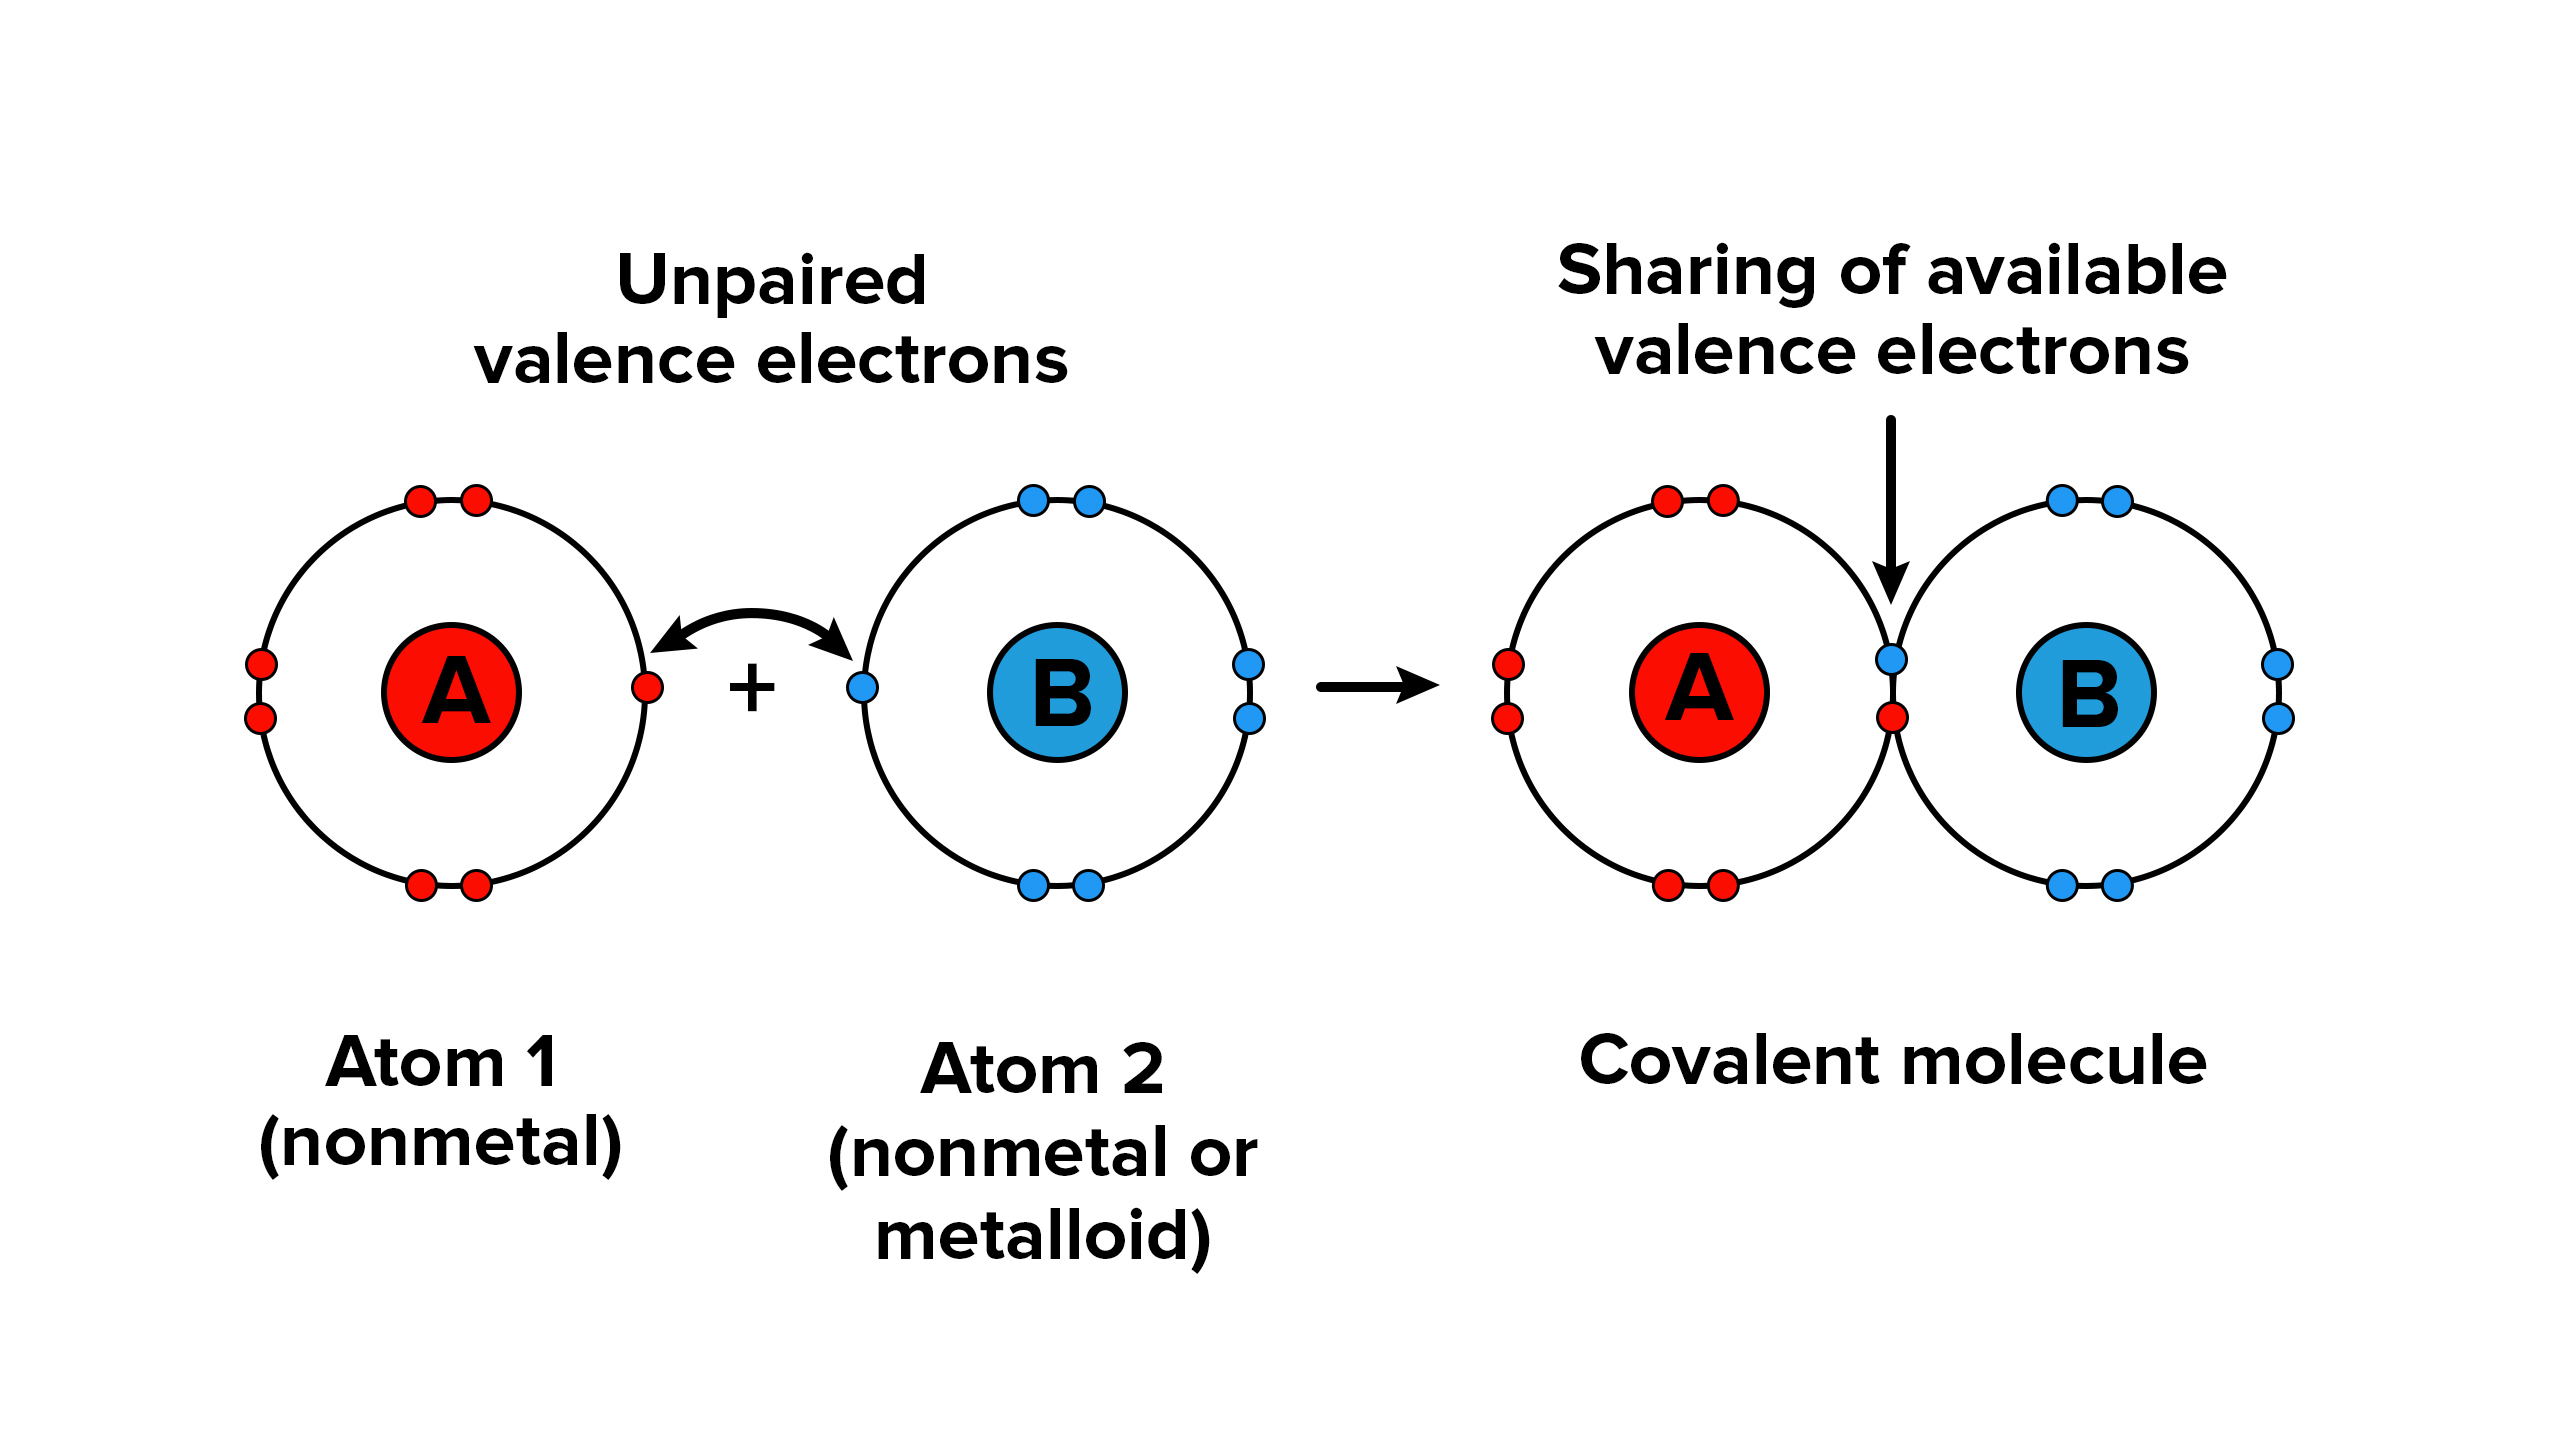
\includegraphics[width=\textwidth]{covalent_bond}
	\caption{Covalent Bond}
\end{figure}

\noindent
Atoms in covalent bonds can have both bonding electrons and non-bonding electrons, where the shared electrons are considered `bonding.' \\

\noindent
\note{Covalent compounds can form single, double, or triple bonds by sharing one, two, or three pairs of electrons, with each bond represented with a straight line.}

\subsection{Molecular Geometry and VSEPR}

\begin{defn}
Molecular Geometry is a description of the three dimensional arrangement of atoms within a molecule, and it plays a critical role in determining the physical and chemical properties of substances.
\end{defn}

\begin{defn}
Valence Shell Electron Pair Repulsion Theory, or VSEPR Theory, is a set of procedures for predicting the geometric structure of a molecule from its lewis dot structure.
\end{defn}

\noindent
In VSEPR, the non-binding electron pairs and the number of atoms bonded to an atom determine the geometric structure of an atom as \textbf{electrons naturally repel each other}. (\note{this is why remembering the number of electron groups is key.}) \\

\noindent
A VSEPR electron group is a group of valence electrons around an atom or molecule. (\note{It is slightly different from an electron pair.})

\subsubsection{The Core of Molecular Geometry based on VSEPR}

\begin{enumerate}
\item Atoms arrange themselves to be as far from other electrons as possible.
\item There is no distinction made between bonding/shared electrons and non-bonding/lone electrons.
\item Single, double, and triple bonds are all counted equally as one pair attached to the central atom.
\end{enumerate}

\subsubsection{Types of VSEPR Configurations}

\begin{figure}[H]
	\centering
	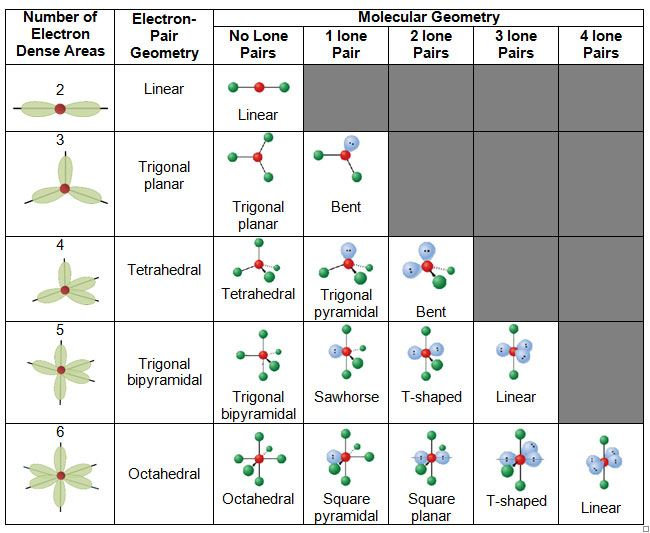
\includegraphics[width=\textwidth]{vsepr_table.jpg}
	\caption{Types of VSEPR Configurations}
\end{figure}

\begin{itemize}
\item Molecules with 2 or 3 VSEPR pairs are \textbf{planar}.
\item Molecules with VSEPR pairs that are strictly $180^\circ$ apart are \textbf{linear}.
\item Molecules with VSEPR pairs that are strictly $120^\circ$ will be \textbf{Triagonal Planar} or \textbf{Angular/Bent}.
\item Molecules with VSEPR pairs that are strictly $109.5^\circ$ will be either \textbf{Tetrahedral,  Trigonal Pyramidal, or Angular/Bent}
\end{itemize}

\begin{table}[H]
\centering
\begin{tabular}{|l|l|l|}
\hline
\textbf{Formula} & \textbf{VSEPR Groups} & \textbf{Shape} \\
\hline
\ce{XB2}   & 2 & Linear \\
\ce{XB3}   & 3 & Trigonal Planar \\
\ce{XB2N1} & 3 & Bent \\
\ce{XB4}   & 4 & Tetrahedral \\
\ce{XB3N1} & 4 & Trigonal Pyramidal \\
\ce{XB2N2} & 4 & Bent \\ 
\hline
\end{tabular}
\caption{X is the Central Atom, B is the Bonding Electron Groups, and N is the Non-Bonding Electron Groups.}
\end{table}

\subsection{Bond Polarity}

The greater the electronegativity of an atom, the greater its electron attraction. By this rule, atoms with different electronegativities will have bonds of different strengths.

\begin{defn}
\textbf{Bond Polarity} is the measure of the magnitude of difference in electron bonds between atoms.
\end{defn}

\begin{itemize}
\item Bonds with equal sharing of electrons are called non-polar covalent bonds.
\item Bonds that do not have an equal sharing of electons are known as polar covalent bonds and are represented with a "D-" or "D+" for negative and positive respectively.
\item Polar covalent bonds create a polarity in the resulting molecule, which influences its resulting properties.
\end{itemize}

\subsubsection{Calculating Bond Polarity}

Electronegativity differences can be used as a rough measure of calculating bond polarity given the following rules:


\begin{table}[H]
\centering
\begin{tabular}{|l|l|}
\hline
\textbf{Electronegativity Range} & \textbf{Bond Polarity Type} \\
\hline
$\Delta \chi < 0.4$ 		& Non-Polar Covalent \\
$0.4 \le \Delta \chi < 2$  	& Polar Covalent \\
$2 \ge \Delta \chi$			& Ionic \\
\hline
\end{tabular}
\caption{$\Delta \chi$ is the magnitude of difference between the electronegativities between the two elements.}
\end{table}

\noindent
For example, Hydrogen has an electronegativity of 2.1 and Chlorine has an electronegativity of 3.0, causing a difference of $\Delta \chi = 0.9$, and thus, a polar covalent bond. \textit{The greater this difference, the higher the polarity.} \\

\noindent
\note{Although the bonds can be polarized, sometimes the polarity can cancel out, causing the molecule to be non-polar.}

\subsection{Molecular Polarity}

\begin{defn}
Molecular Polarity is a measure of degree inequality in the attractiong of bonding electrons to various locations within a molecule, where polar molecules have unsymmetrical charge distribution and non-polar molecules have symmetrical charge distribution.
\end{defn}

\noindent
\note{Molecular geometry and bond polarity combined determine molecular polarity.}

\section{Lecture 2: Naming of Compounds}

The International Union of Pure and Applied Chemistry, or IUPAC, sets the following standard rules for naming compounds in chemistry.

\begin{itemize}
\item \textbf{Binary Ionic Compounds} contain a metal and a non-metal.
\item \textbf{Binary Molecular Compounds} consist of only non-metals. (\note{For naming purposes, metalloids are treated as non-metals.})
\item \textbf{Binary Acids} are compounds that release hydrogen ions when dissolved in water.
\end{itemize}

\subsection{Ionic Compounds}

\begin{itemize}
\item Ionic Compounds are the attraction between oppositely-charged ions, not atoms.
\item Ionic compounds form crystal lattices, not molecules.
\item The charge on an ionic compounds is always neutral.
\item Ionic compounds may contain one or more \textit{polyatomic ions.}
\end{itemize}

\subsubsection{Metal Ions}

\noindent
For naming purposes, there are two types of metal ions: fixed and variable charge.

\begin{defn}
\textbf{Fixed charge} ions are metal ions that form one type of positive ion that always have the same charge. \textbf{Variable charge} ions are metal ions that can form more than one type of positive ion.
\end{defn}

\noindent
The only fixed-charge ions are the metal elements in the IA, IIA, IB, IIB, and IIIA groups, or Lithium, Sodium, Potassium, Rubidium, Cesium, Beryllium, Magnesium, Calcium, Strontium, Barium, Aluminum, Gallium, Silver, Zinc, and Cadmium. \textit{All other metals have variable charge}, such as Chromium, Cobalt, or Gold.

\subsection{Naming Binary Ionic Compounds}

\begin{itemize}
\item When naming ionic compounds, positively-charged ions (cations) are named first, and negatively-charged ions (anions) are named after.
\item Metal ions (fixed or variable) take the name of the metal they come from.
\item Non-metal ions are named by taking the stem of the non-metal and adding the suffix "-ide."
\end{itemize}

\begin{example}
\ce{Li+} is a Lithium Ion, \ce{Mg^{2+}} is a Magnesium Ion, but \ce{Fl-} is a Fluoride ion and \ce{O^{2-}} is an Oxide ion.
\end{example}

\noindent
\note{Polyatomic ions always bring their own name to the compound.}

\begin{table}
\centering
\begin{tabular}{|l|l|l|l|}
\hline
\textbf{Element} & \textbf{Stem} & \textbf{Name of Ion} & \textbf{Formula} \\
\hline
Bromine   	& brom-	  & bromide   ion & \ce{Br-} \\
Carbon    	& carb-   & carbide   ion & \ce{C^{4-}} \\
Chlorine  	& chlor-  & chloride  ion & \ce{Cl-} \\
Fluorine	& fluor-  & fluoride  ion & \ce{F-} \\
Hydrogen	& hydr-   & hydride   ion & \ce{H-} \\
Iodine		& iod-    & iodide    ion & \ce{I-} \\
Nitrogen	& nitr-   & nitride   ion & \ce{N^{3-}} \\
Oxygen		& ox-	  & oxide 	  ion & \ce{O^{2-}} \\
Phosphorus 	& phosph- & phosphide ion & \ce{P^{3-}} \\
Sulfur		& sulf-   & sulfide   ion & \ce{S^{2-}} \\
\hline
\end{tabular}
\caption{Names for Common Non-Metal Ions}
\end{table}

\begin{example}
\ce{CaF2} would be Calcium flouride, and no importance is placed on the amount fo each element. 
\end{example}

\noindent
When naming binary ionic compounds with variable-charge metals, there has to be a differentiation between the different charges of the metal for situations such as differentiating between \ce{FeS} and \ce{Fe2S3} given the ions \ce{Fe^{2+}} and \ce{Fe^{3+}}.

\noindent
The solution to this is referring to each ion of the metal by its cation charge in roman numerals within parentheses, so \ce{Fe^{2+}} becomes Iron (II) and \ce{Fe^{3+}} becomes Iron (III).

\noindent
\note{If there is a metal in the compound, the metal is ionic.}

\subsection{Naming Compounds with Polyatomic Ions}

\begin{enumerate}
\item Most polyatomic ions are negatively charged, and the only two main positive ones are ammonium and hydonium.
\item Four polyatomic ions have names that end in "-ide" already: hydroxide, cyanide, azide, and peroxide.
\item Pay attention to the "-ate" and "-ite" pairs, as htey differ by the number of oxygen atoms, where "-ate" always has a greater number of oxygen atoms. For example, Sulfate (\ce{SO4^2-}) and Sulfite (\ce{SO3^2-}).
\item Some pairs differ by the addition of a hydrogen ion, such as Carbonate (\ce{CO3^2-}) and Hydrogen Carbonate (\ce{HCO3^2-}).
\item When Sulfur replaces an Oxygen atom, the prefix "Thio-" is added to the name, such as with Cyanate (\ce{OCN}) and Thiocyanate (\ce{SCN}) or Sulfate (\ce{SO4^2-}) and Thiosulfate (\ce{S2O3^2-}).
\end{enumerate}

\subsection{Binary Molecular Compounds}

Binary molecular compounds consist of two non-metal elements, and these compounds are named as the formula is written.

\begin{itemize}
\item The least electonegative element is named first.
\item The stem of the second non-metal follows with the suffix "-ide."
\item Numerical prefixes are used to indicate the number of both atoms present.
\end{itemize}

\noindent
\note{The number of atoms present is not clarified for polyatomic ions, but it is for binary molecular compounds.}

\begin{table}[H]
\centering
\begin{tabular}{|c|c|}
\hline
\textbf{Prefix} & \textbf{Value} \\
\hline
mono & 1 \\
di & 2 \\
tri & 3 \\
tetra & 4 \\
penta & 5 \\
hexa & 6 \\
hepta & 7 \\
octa & 8 \\
nona & 9 \\
deca & 10 \\
\hline
\end{tabular}
\end{table}

\noindent
\note{The exception to this rule is that binary compounds with hydrogen listed as the first element are named without using the prefix for how many atoms there are, and the prefix "mono" is always dropped at the beginning of a name.}

\subsubsection{Common Names to Know}

\begin{table}
\centering
\begin{tabular}{|l|l|}
\hline
\textbf{Formula Unit} & \textbf{Name} \\ 
\hline
\ce{H2O}  & Water \\
\ce{H2O2} & Hydrogen Peroxide \\
\ce{NH3}  & Ammonia \\
\ce{N2H4} & Hydrazine \\
\ce{CH4}  & Methane \\
\ce{C2H6} & Ethane \\
\ce{PH3}  & Phosphine \\
\ce{AsH3} & Arsine \\
\hline
\end{tabular}
\end{table}

\noindent
\note{The above examples are all binary compounds, but other molecular compounds with more than 2 elements don't follow these rules.} \\

\subsection{Introduction to Acids}

\begin{defn}
An acid is a hydrogen-containing molecular compound whose molecules yield Hydrogen ions (\ce{H+}) when dissolved in water (\ce{H2O}).
\end{defn}

\noindent
These acids can be identified by having Hydrogen as the first element shown in its formula, such as \ce{HCl}, \ce{H2S}, \ce{H2SO4}, or \ce{HNO3} (which are all acids), whereas \ce{NH3}, \ce{CH4}, \ce{PH3}, or \ce{SiH4} are all non-acidic. \\

\noindent
\note{Acids produce \ce{H+} in water, but an anion is also produced, depending on the structure of the molecular compound. For example, \ce{HCl} produces \ce{H+} and \ce{Cl-}.}

\subsubsection{Acid Nomenclature}

\begin{table}[H]
\centering
\begin{tabular}{|c|l|}
\hline
\textbf{Anion Ending} & \textbf{Acid Name} \\
\hline
"-ide" & hydro-\textit{(stem)}-ic acid \\
"-ate" & \textit{(stem)}-ic acid \\
"-ite" & \textit{(stem)}-ous acid \\
\hline
\end{tabular}
\end{table}

\subsection{Common Student Mistakes}

\begin{itemize}
\item For \textbf{ionic compounds ONLY}, formulas \textbf{must be reduced to its simplest ratios}. For example, \ce{Mn2O4} must be reduced to \ce{MnO2}.
\item Do not confuse Ammonia (\ce{NH3}) and an Ammonium Ion (\ce{NH4+}).
\item Chemical formulas do not show ionic charges. For example, write table salt as  \ce{NaCl}, not \ce{Na^{+}Cl^{-}}.
\item Don't put parentheses unless they are needed to show more than one of the same ion. For example, write \ce{NaNO3}, not \ce{Na(NO3)}
\end{itemize}


